\documentclass{article}

% Language setting
\usepackage[spanish]{babel}

% Set page size and margins
\usepackage[a4paper,top=2cm,bottom=2cm,left=3cm,right=3cm,marginparwidth=1.75cm]{geometry}
\setlength{\parindent}{0pt}
\setlength{\parskip}{3.5pt}
% Useful packages
\usepackage{amsmath}
\usepackage{graphicx}
\usepackage[colorlinks=true, linkcolor=black, urlcolor=blue]{hyperref}
\usepackage{tikz}
\usepackage{listings}


% Uncomment these packages if you want to use dark mode
% \usepackage{darkmode}
% \enabledarkmode

% Title and author
\title{Tarea 1 - Redes de Banda Ancha}
\author{Álvaro Hernández Riquelme, DNI: 49339705J}
\date{\today}

\begin{document}

%%%%%%%%%%%%%%%%%%%%%%%%%%%%%%%%%%

\maketitle
\tableofcontents
\newpage


%%%%%%%%%%%%%%%%%%%%%%%%%%%%%%%%%%

\section{Tarea 1}

\subsection{¿Qué comando crea la LAN?}

El comando que crea la LAN, como está en el código a partir de la \textbf{línea 51}, es:

\begin{verbatim}
    set lan [$ns newLan $nodelist $opt(bw) $opt(delay) \
             -llType $opt(ll) -ifqType $opt(ifq) \
             -macType $opt(mac) -chanType $opt(chan)]
\end{verbatim}

Crearía la LAN e inicializaría los parámetros necesarios,

\subsection{¿Cual es la velocidad (bandwidth) de la LAN?}

En la \textbf{línea 03} del código, se ve configurado el bandwith de la LAN a 10Mbps:

\begin{verbatim}
    set opt(bw) 10Mb
\end{verbatim}

\subsection{¿Cuál es el tamaño (bytes) que usamos en el tráfico generado y el intervalo entre eventos de transmisión de paquetes?}

En la \textbf{línea 81} del código, se ve configurado el tamaño de los paquetes a \textbf{1000 bytes}:

\begin{verbatim}
    $cbr_($i) set packetSize_ 1000
\end{verbatim}

Después de esta línea, tenemos un rate especificado (que será la frecuencia) entre eventos de paquetes cbr, que está a \textbf{644kbps}:

\begin{verbatim}
    set rate 644k
    $cbr_($i) set rate_ $rate
\end{verbatim}

\subsection{¿Cuál es la duración de la simulación con tráfico activo?}

En la \textbf{línea 02} se crea una variable fin con el valor de \textbf{10.5 segundos}, y otra variable start con el valor de \textbf{0.5 segundos}, por lo que el tiempo de simulación con tráfico activo será de 10 segundos.

\begin{verbatim}
    set opt(fin) 10.5;
    $ns at 0.5 "$cbr_($i) start"
    $ns at $opt(fin) "$cbr_($i) stop"
\end{verbatim}

\subsection{Ejecución de la simulación}

Al ejecutar la simulación, con el comando \verb|ns tarea1.tcl -nn 4 -seed 1440|, se abrirá el visualizador nam con la simulación de la red:
\newpage
\begin{figure}[h]
	\centering
	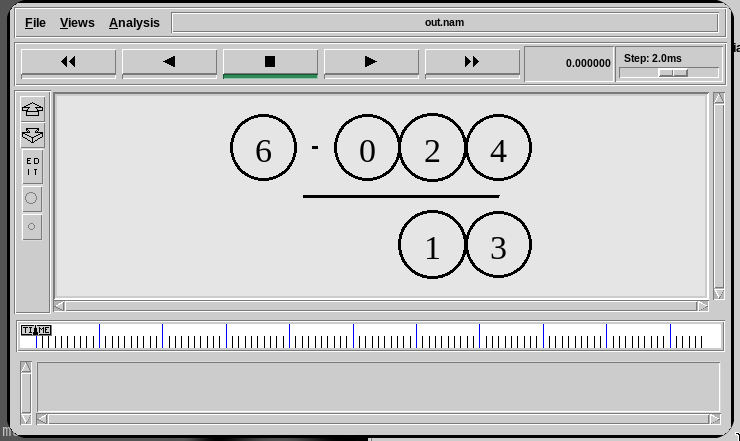
\includegraphics[width=0.6\textwidth]{src/outnam.png}
	\caption{Salida de la simulación}
\end{figure}

Donde los nodos del 1 al 4 son los nodos definidos y que generarán tráfico, el
nodo 0 es el sumidero del tráfico generado y los nodos 5 y 6 serán auxiliares de NS. Además del visualizador nam con el \textbf{out.nam}, también se generará un archivo de trazas tipo trace \textbf{csmacd.tr} con los datos de la simulación.

Se puede analizar una línea de las trazas generadas para mostrar el formato:

\begin{verbatim}
    r 0.501083 5 0 cbr 1000 ------- 0 1.0 0.0 0 0
\end{verbatim}

Donde, en este caso:
\begin{itemize}
	\item \textbf{r} significa paquete recibido, será el tipo de evento, en nuestro archivo será +,-, r,h o d.
	\item \textbf{0.501083} es el instante que ocurre el evento
	\item \textbf{5} es el nodo que envía el paquete
	\item \textbf{0} es el nodo que recibe el paquete
	\item \textbf{cbr} es el tipo de tráfico: constant bit rate
	\item \textbf{1000} es el tamaño del paquete
	\item \textbf{-----} son las flags
	\item \textbf{0} es el identificador de flujo
	\item \textbf{1.0} es el identificador del nodo fuente
	\item \textbf{0.0} es el identificador del nodo destino
	\item \textbf{0} es el número de secuencia
	\item \textbf{0} es el identificador de paquete, único para cada paquete creado en una simulación NS
\end{itemize}

\subsection{¿Cuál es el total de paquetes recibidos (P) correctamente en el receptor?}


Viendo el archivo de trazas, se puede extraer cuales serían los paquetes recibidos correctamente, serían los que empiezan por la letra \textbf{r}. Bastaría con filtrar las líneas de trazas que empiecen por \textbf{r}, se usará un \textbf{script de awk} para ello:


\begin{verbatim}
BEGIN {
    received = 0;
}
{
    if ($1 == "r") {
        received++;
    }
}
END {
    printf "%d", received;
}
\end{verbatim}

El programa devuelve que se ha recibido un total de \textbf{3220} paquetes correctamente.

\subsection{¿Cuál es el total de paquetes descartados (por las estaciones) durante la simulación?}

Hemos visto que en nuestra simulación hay 4 nodos que generan tráfico. Como todos los nodos envían al nodo 0, y están en un medio compartido, por cada envío hay otros tres nodos que reciben esa información, y al no ser el destinatario (Siempre será el nodo 0) se descartarán esos paquetes.

Es decir, por el funcionamiento de \textbf{CSMA CD} y la cantidad de nodos en la simulación se descartarán tres paquetes por cada paquete enviado. Si han habido 3220 paquetes enviados, la cantidad de paquetes descartados será de \textbf{9660 paquetes.}

\subsection{¿Cuál es el porcentaje de paquetes descartados en una estación transmisora de paquetes?}

En la pregunta anterior se ha visto que para cada paquete enviado, se descartan tres. Y como las estaciones transmisoras tienen el mismo rate de envío, se podría decir que hay 3/4 de paquetes descartados por estación. un \textbf{75\%.}

\subsection{¿Cuál es el throughput y la eficiencia del sistema?}

Como son 3220 los paquetes enviados correctamente, a 1000 bytes por paquete, y 8 bits por cada byte, dividido por el tiempo de simulación:

\[ T = \frac{3220 \cdot 1000 \cdot 8}{10} = 2576000 \text{ bps} \]

Por lo que el throughput del sistema será de ~\textbf{ 2.58 Mbps}

La eficiencia vendrá definida como la división entre el throughput y la velocidad de la LAN, que se ha visto anteriormente que era 10Mbps. Por lo que, teniendo el throughput, será:

\[E = \frac{T}{v} = \frac{2576000}{10000000} = 0.2576
\]

Por lo que la eficiencia será del \textbf{25,8}\% aproximadamente. No es del 100\% debido a las colisiones, descartes, retardos y el algoritmo de backoff que pueda haber en cada envío.

\subsection{Throughput de los nodos 1,2,3,4.}

Ya que se envían 3220 paquetes, y el rate es el mismo para todos, se puede afirmar que cada nodo envía \(\frac{3220}{4} = 805 \) paquetes. Esto se puede asumir porque no hay paquetes dropped (d). Para ejercicios posteriores, habrá que filtrar cuantos paquetes envía cada nodo.

Aunque se pueda directamente repartir el throughput calculado anteriormente entre 4 para cada nodo, podemos comprobarlo por separado para los paquetes que envían:

$$\frac{805 \cdot 1000 \cdot 8}{10} = 644000 \text{ bps} $$

Por lo que el throughput de cada nodo será de \textbf{ 0.644 Gbps}

\subsection{Realice un trazado de eventos de los nodos 1 a 4.}

En el inicio, en 0.5, se generan los paquetes desde los nodos 1 al 4, e intentarán enviar cada uno de ellos su paquete al nodo 5 (atención a columnas 3 y 4):

\begin{verbatim}
h 0.5 1 5 cbr 1000 ------- 0 1.0 0.0 0 0
h 0.5 2 5 cbr 1000 ------- 0 2.0 0.1 0 1
h 0.5 3 5 cbr 1000 ------- 0 3.0 0.2 0 2
h 0.5 4 5 cbr 1000 ------- 0 4.0 0.3 0 3
\end{verbatim}

Como no hay congestión, en el instante 0.5001 entran y salen directamente de la cola estos paquetes:

\begin{verbatim}
+ 0.5001 1 5 cbr 1000 ------- 0 1.0 0.0 0 0
- 0.5001 1 5 cbr 1000 ------- 0 1.0 0.0 0 0
        .           .           .
        .           .           .
        .           .           .
- 0.5001 4 5 cbr 1000 ------- 0 4.0 0.3 0 3
\end{verbatim}

Ahora es cuando puede ocurrir colisión, aunque el primer paquete generado por el nodo 1 sí se recibe sin problemas el primero:

\begin{verbatim}
r 0.501083 5 0 cbr 1000 ------- 0 1.0 0.0 0 0
\end{verbatim}

Después, debería llegar el paquete generado por el segundo nodo, pero \textbf{colisiona} con el que genera el tercer nodo, ganando éste último la contienda, por lo que el segundo nodo entra en el periodo de \textbf{backoff} y mientras tanto, se reciben los paquetes generados por los nodos 3, y le da tiempo también al 4 mientras el backoff del 2, finalmente llega el paquete del nodo 2.

\begin{verbatim}
r 0.502198 5 0 cbr 1000 ------- 0 3.0 0.2 0 2
r 0.50495 5 0 cbr 1000 ------- 0 4.0 0.3 0 3
r 0.506589 5 0 cbr 1000 ------- 0 2.0 0.1 0 1
\end{verbatim}


\subsection{Calcule el retardo de propagación de los estaciones 1, 2, 3 y 4.}

Como dice el enunciado de la pregunta, el retardo de propagación se calculará midiendo la diferencia entre el instante de tiempo que corresponde al envío del paquete y el instante de tiempo en el que el paquete se recibe en la estación de destino.

Para ello, filtraremos las 8 primeras líneas que tengan la acción \textbf{"h"} y \textbf{"r"} (dos paquetes por cada nodo) con el script de awk \textbf{filtroretardos}.
Lo que hace este script será hacer una variable \verb|action = $1| y otras \verb|receive_count y send_count| para controlar el resultado que buscamos, al ejecutar el script devuelve:
\begin{verbatim}
h 0.5 1 5 cbr 1000 ------- 0 1.0 0.0 0 0
h 0.5 2 5 cbr 1000 ------- 0 2.0 0.1 0 1
h 0.5 3 5 cbr 1000 ------- 0 3.0 0.2 0 2
h 0.5 4 5 cbr 1000 ------- 0 4.0 0.3 0 3
r 0.501083 5 0 cbr 1000 ------- 0 1.0 0.0 0 0
r 0.502198 5 0 cbr 1000 ------- 0 3.0 0.2 0 2
r 0.50495 5 0 cbr 1000 ------- 0 4.0 0.3 0 3
r 0.506589 5 0 cbr 1000 ------- 0 2.0 0.1 0 1
h 0.512422 1 5 cbr 1000 ------- 0 1.0 0.0 1 4
h 0.512422 2 5 cbr 1000 ------- 0 2.0 0.1 1 5
h 0.512422 3 5 cbr 1000 ------- 0 3.0 0.2 1 6
h 0.512422 4 5 cbr 1000 ------- 0 4.0 0.3 1 7
r 0.513471 5 0 cbr 1000 ------- 0 4.0 0.3 1 7
r 0.514483 5 0 cbr 1000 ------- 0 2.0 0.1 1 5
r 0.515478 5 0 cbr 1000 ------- 0 1.0 0.0 1 4
r 0.516303 5 0 cbr 1000 ------- 0 3.0 0.2 1 6
\end{verbatim}

Estas son todas las trazas que harán falta para el cálculo. Para cada nodo, importará la columna 3 cuando el evento es \textbf{h}, que indicará quién envía el paquete y la 9 cuando sea \textbf{r}, indicará qué nodo envió el mensaje inicialmente.
Filtrando los dos primeros paquetes del nodo 1, se podrá calcular el retardo observando los tiempos de envío \(t_h\) y recepción \(t_r \), siendo las \textbf{filas 1,5,9, y 15} del output las relevantes:

\[r = t_r - t_h\]

Se sustituye en el nodo 1 y se hace la media de los dos retardos:

\[
	r_{1} = \frac{(0.501083 - 0.5) + (0.515478 - 0.512422)}{2} = 0.0020694999999999464s
\]

Ahora, repetiremos lo mismo para los demás nodos. Al ser pocos nodos y únicamente dos paquetes, se puede filtrar manualmente desde el output recibido del script \textbf{filtroretardos.awk}, en caso de más paquetes, se hubiera necesitado ampliar el script para el cálculo automático.

\[
	r_{2} = \frac{(0.506589 - 0.5) + (0.514483 - 0.512422)}{2} = 0.004324999999999968s
\]

\[
	r_{3} = \frac{(0.502198 - 0.5) + (0.516303 - 0.512422)}{2} = 0.0030394999999999728s
\]

\[
	r_{4} = \frac{(0.50495 - 0.5) + (0.513471 - 0.512422)}{2} = 0.0029994999999999883s
\]

\subsection{Calcule la Utilización del Canal U}

Primero se usará la cantidad de paquetes para obtener el tiempo que tarda para transmitir todos nuestros paquetes a una velocidad constante en la lan. En este caso, la velocidad de la lan es de 10Mbps, por lo que el tiempo que tarda en transmitir 3220 paquetes de 1000 bytes es de:

\[
    \frac{3220 \cdot 8 \cdot 1000}{10 \cdot 10^6} = 2.576s
\]

Ahora ese tiempo, se dividurá entre el tiempo total de la simulación, que es de 10.5 segundos, para obtener la utilización del canal:

\[
    U = \frac{2.576}{10.5} = 0.24533
\]

Por lo que la utilización del canal es de \textbf{24.533\%.}

\subsection{Calcule la Tasa de Colisiones (NO RESPONDE)}

La tasa de colisiones se calculará dividiendo el número de colisiones entre el número total de paquetes enviados.

(nota: la única forma que se me ocurre de encontrar las colisiones es observar si los paquetes recibidos se reciben al mismo orden que los enviados. No sabría pasarlo a awk).

\textbf{NO RESPONDE.}

\newpage
\section{Ejercicio 2.}

\subsection{Ejecución del script.}

Se hará un script de bash que recorrerá un bucle ejecutando la simulación con la semilla indicada en el enunciado. En este caso \textbf{4933}.

\begin{verbatim}
#!/bin/bash

for i in {1..21}; do
    ns tarea1.tcl -nn $i -seed 4933
done
\end{verbatim}

El bucle va desde 1 hasta 21 pasado como argumento de nodos su índice y la semilla constante de 4933. También se ha modificado el archivo de simulación \textbf{tcl} para que pueda generar las trazas en archivos distintos. La línea \textbf{115} quedará como:

\begin{verbatim}set tracefd     [open "csmacd_n$opt(nn).tr" w]\end{verbatim}

De este modo se generarán los 21 archivos de traza.

\subsection{Filtrar los resultados por lotes}

Para filtrar todos los archivos, se hará otro \textbf{script de bash} que ejecute los distintos \textbf{scripts de awk} que han hecho falta para cada archivo, y los concentre en \textbf{statistics.dat}.

El script de \textbf{throughput.awk} calculará tanto el throughput como la eficiencia y utilización, de forma similar a la que se hace en el ejercicio 1. El script de \textbf{dropped.awk} filtrará las líneas que empiecen por d, y sumará uno por cada línea filtrada.

Ambos scripts responden únicamente con el resultado para poder cumplir el formato que se pide. El script de bash \textbf{createstats.sh} ejecutará ambos scripts awk para todos los \textbf{csmacd\_ni.tr} e imprimirlo en nuestro archivo dat.

\subsection{Resultado y figuras.}

Para generar las figuras, se usará el paquete \textbf{TikZ} de \LaTeX, siendo bastante similar todos los archivos .tex, pero cambiarán los valores \textbf{ymax y xmax. }. El código .tex accede a statistics.dat, por lo que también cambiará la columna de referencia para el eje x en cada figura. El eje y serán los nodos para todas las figuras.
\newpage
\subsubsection{Throughput}

El throughput podemos observar que se mantiene una subida lineal conforme van habiendo más nodos, hasta el nodo 16, donde hay cada vez menos diferencia en la subida. Esto se debe a que el canal ya está saturado y no puede transmitir más paquetes.

\begin{figure}[h]
	\centering
	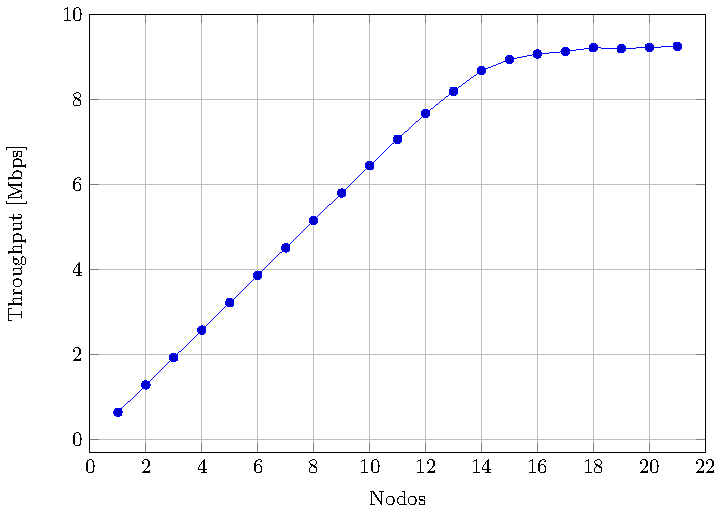
\includegraphics[width=0.7\textwidth]{src/Throughput.pdf}
	\caption{Throughput de la LAN con 21 nodos.}
\end{figure}

\subsubsection{Eficiencia}
La eficiencia seguirá el mismo patrón que el throughput, ya que es la relación entre el throughput y el ancho de banda. Por lo que también se estabilizará a partir del nodo 16.
\begin{figure}[h]
    \centering
    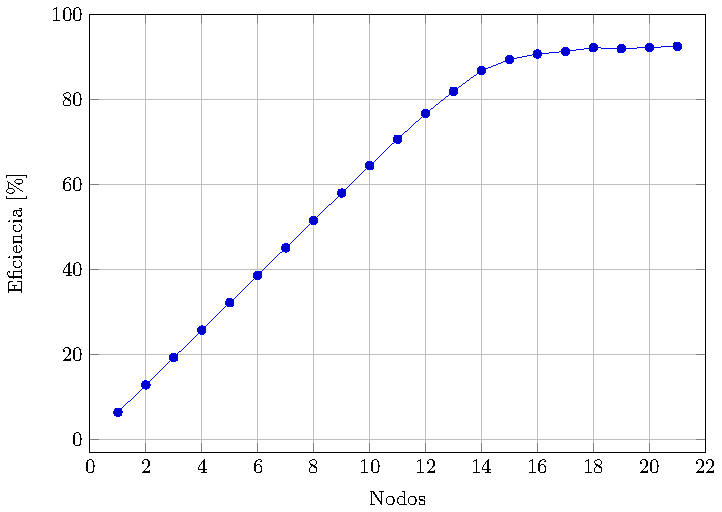
\includegraphics[width=0.7\textwidth]{src/Efficiency.pdf}
    \caption{Eficiencia de la LAN con 21 nodos.}
\end{figure}
\newpage
\subsubsection{Utilización}

El cálculo de la utilización es bastante similar al de la eficiencia, por lo que sigue el mismo patrón pero será un poco menor.

\begin{figure}[h]
    \centering
    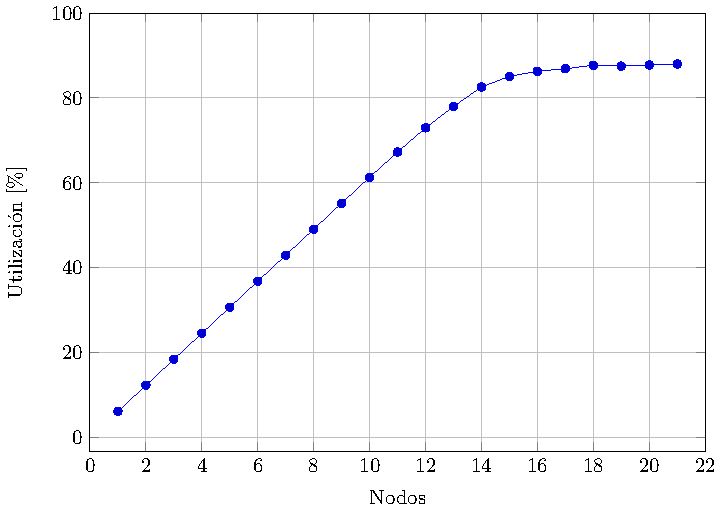
\includegraphics[width=0.7\textwidth]{src/Utilization.pdf}
    \caption{Eficiencia de la LAN con 21 nodos.}
\end{figure}

\subsubsection{Pérdida de paquetes}

A partir del nodo 14 empieza a haber una pérdida de paquetes considerable, y a partir del nodo 16 se dispara. Esto se debe a que el canal ya no puede transmitir más paquetes y se empiezan a perder. Coincide con el punto donde se estabiliza el throughput y la eficiencia al no aumentarse los paquetes enviados con éxito, sino que se aumentan los perdidos.

\begin{figure}[h]
    \centering
    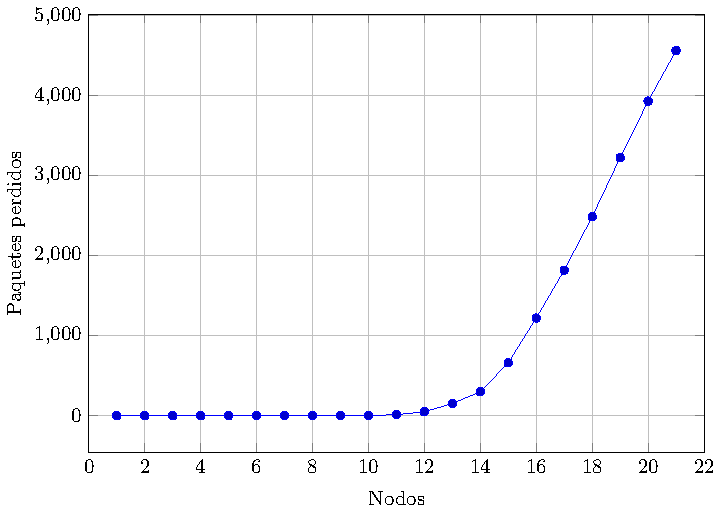
\includegraphics[width=0.7\textwidth]{src/Dropped.pdf}
    \caption{Pérdida de paquetes de la LAN con 21 nodos.}
\end{figure}

\subsection{¿Cuál es el porcentaje medio de pérdida de paquetes que experimentaría una estación cuando la LAN tiene 12 y 21 estaciones?}

En este caso, mirando la tabla de \textbf{statistics.dat}, tendremoa que la LAN con 12 nodos experimentará una pérdida de \textbf{49 paquetes}, y la LAN con 21 experimentará una pérdida de \textbf{4566 paquetes.}

Por lo que, para el porcentaje, se dividirá entre la cantidad de paquetes enviados (h). Se usará el script \textbf{enviados.awk} para ver la cantidad enviada en cada uno. Una vez ejecutado, será de 9672 y 16926. Llamaremos \(dp_i\) al porcentaje de paquetes perdidos \textbf{dropped percentage}.

\[dp_{12} = \frac{d_{12}}{h_{12}} = \frac{49}{9672} = 0.005 = 0.5\% \]

\[dp_{21} = \frac{d_{21}}{h_{21}} = \frac{4566}{16926} = 0.26976 \approx 27\% \]

\section{Ejercicio 3}

\subsection{Throughput de la simulación con 21 nodos.}

Como se sigue usando la semilla de los 4 primeros dígitos del DNI, se copiará el archivo de trazas de 21 nodos \textbf{csmacd21.tr}, y se trabajará con sus trazas. Se realizará un \textbf{script de awk} llamado \textbf{separate\_throughputs.awk}, donde se calcularán los throughputs por separado de cada nodo. Se exportará en \textbf{lan\_21nodos.dat} con una columna siendo la cantidad de nodos, y la otra el throughput.

\begin{figure}[h]
	\centering
	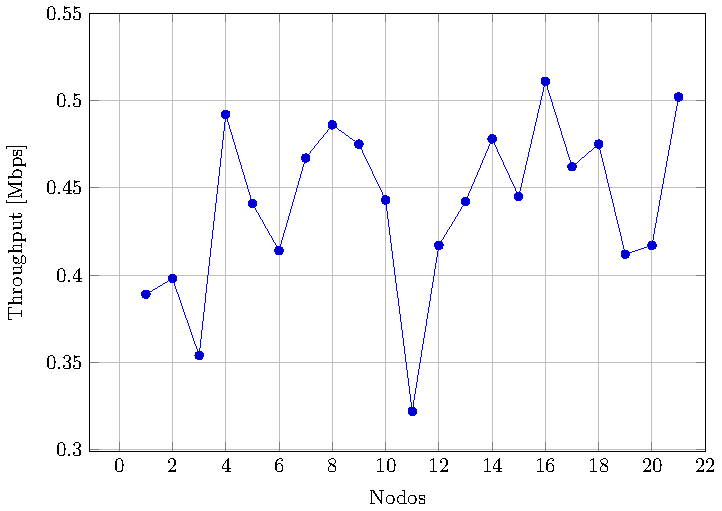
\includegraphics[width=0.7\textwidth]{src/main.pdf}
	\caption{Throughput de la LAN con 21 nodos.}
\end{figure}


Aunque parezca que el throughput tiene bastante variabilidad, en realidad no tiene una desviación muy grande, ya que el rango de valores estaría comprendido entre 0.3 y 0.55 aproximadamente. Por lo que se puede suponer que el throughput está correctamente repartido.

\subsection{Indice de Jain}

En este caso, para procesar el archivo \textbf{lan\_21nodos.dat}, se usará un script en \textbf{Python} que calcule el índice de Jain. Se llamará \textbf{jain.py}. En nuestro caso, el límite de nodos es 21 y al throughput lo llamamos \(T_i\).

\[J = \frac{\left( \sum_{i=1}^{21} T_i \right)^2}{21 \sum_{i=1}^{21} T_i^2}\]

La forma de calcularlo será sencilla, una vez filtrados los throughputs y añadidos en un array, se dividirá por numerador y divisor con su respectivo sumatorio.Y una vez calculado ambos se dividirá.

El cálculo será el siguiente:

\newpage

\begin{verbatim}
# Recibe throughputs que será un array
def calculate_jain_index(throughputs):
    n = len(throughputs)
    sum_throughput = 0
    # Bucle del numerador, los suma todos y luego lo eleva al cuadrado.
    for x in throughputs:
        sum_throughput += x
    numerator = sum_throughput ** 2

    sum_squared = 0
    # Bucle del denominador, suma todos los cuadrados. Luego producto con n.
    for x in throughputs:
        sum_squared += x ** 2
    denominator = n * sum_squared

    return numerator / denominator
\end{verbatim}

El resultado del script es de \textbf{0.9885}. Por lo que se puede considerar que la red es bastante justa en cuanto a la distribución de los nodos.

\end{document}
